% Tipo di documento. L'uso di twoside implica che i capitoli inizino sempre con la prima pagina a sinistra, eventualmente lasciando una pagina vuota nel capitolo precedente. Se questa cosa è fastidiosa, è possibile rimuoverlo. 
\documentclass[a4paper,openright]{report}

% Dimensione dei margini
\usepackage[a4paper,top=3cm,bottom=3cm,left=3cm,right=3cm]{geometry} 
% Dimensione del font
\usepackage[fontsize=12pt]{scrextend}
% Lingua del testo
\usepackage[italian,english]{babel}
% Lingua per la bibliografia
% \usepackage[fixlanguage]{babelbib}
% Codifica del testo
\usepackage[utf8]{inputenc} 
% Font mono (quello di default non supporta il grassetto)
\usepackage{courier}
% Encoding del testo
\usepackage[T1]{fontenc}
% Lorem Ipsum
\usepackage{lipsum}
% Bibliografia
\usepackage[
backend=biber,
bibstyle=other/custom-numeric,
citestyle=numeric,
sorting=none,
]{biblatex}
% Sorgente della bibliografia
\addbibresource{chapters/Bibliography.bib}
% Per ruotare le immagini
\usepackage{rotating}
% Per cambiare i capitoli
\usepackage{titlesec}
\titleformat{\chapter}[hang]
  {\normalfont\bfseries\huge}{\thechapter}{1em}{\huge}
% Per mostrare nell'indice anche le subsubsection
\setcounter{tocdepth}{3}
% Per modificare l'header delle pagine 
\usepackage{fancyhdr}
% Librerie matematiche
\usepackage{amssymb}
\usepackage{amsmath}
\usepackage{mathtools}
\usepackage{amsthm}         
% Uso delle immagini
\usepackage{graphicx}
% Uso dei colori
\usepackage[dvipsnames,svgnames,x11names]{xcolor}
% Uso dei listing per il codice
\usepackage{listings}          
% Per inserire gli hyperlinks tra i vari elementi del testo 
% \usepackage[hang, flushmargin]{footmisc}
% Diversi tipi di sottolineature
\usepackage[normalem]{ulem}
% Fix relative indenting
\usepackage{lstautogobble}
% Code coloring
\usepackage{color}
% Nice font
\usepackage{zi4}
% Loads the Latin Modern font
\usepackage{lmodern}
% For text alignment
\usepackage{ragged2e}
% Customizes the appearance of figure and table captions
\usepackage{caption}
% Code highlighting
\usepackage[newfloat,outputdir=out]{minted}
% Better frame for minted
\usepackage{tcolorbox}
\tcbuselibrary{minted,skins,breakable,xparse}
\tcbuselibrary{listingsutf8} % Allows minted in tcolorbox
% Additional options to control the placement of figures and tables
\usepackage{float}
% No paragraph indentation instead vspaces
\usepackage[skip=5pt]{parskip}
% Allows customization of line spacing
\usepackage{setspace}
% Enables switching or substituting hyphenation patterns in your document
\usepackage{hyphsubst}
% Improves the overall typography of the document by subtly adjusting spacing and font shapes
\usepackage{microtype}
% Allows the creation of hyperlinks in the document
\usepackage{hyperref}
% Adds back-references from footnotes to the point in the text where the footnote was used
\usepackage{footnotebackref}
% Tools for formatting and managing quotes in your document
% To be used after minted
\usepackage{csquotes}
% Adding sub-captions to figures and tables
\usepackage{subcaption}
% Drawing electrical and electronic circuit diagrams
\usepackage{circuitikz}
% Permits to patch macros
\usepackage{xpatch}

\usepackage{multirow}
\usepackage{booktabs}
\usepackage{siunitx} % For proper unit formatting
\usepackage{cleveref} % For proper unit formatting


% Comments ( substitute command name and name )
\newcommand{\cuno}[1]{\textcolor{red}{[\bfseries Persona 1: #1]}}
\newcommand{\cdue}[1]{\textcolor{red}{[\bfseries Persona 2: #1]}}

% Don't include in \leftmark "Chapter"
\renewcommand{\chaptermark}[1]{%
  \markboth{\thechapter. #1}{}%
}
% Modifica lo stile dell'header
\pagestyle{fancy}
\fancyhf{}
% These work if the document is in twoside mode
% \fancyhead[CE,CO]{\rightmark}
% \fancyhead[LE,RO]{\textbf{\thepage}}

% Make the header
% on the left side, show the chapter title if no section is present, otherwise the section title
% on the right side, show the page number
\fancyhead[L]{
  \ifnum\value{section}=0 % Check if no section exists
    \leftmark            % Use Chapter title
  \else
    \rightmark           % Use Section title
  \fi
}
\fancyhead[R]{\textbf{\thepage}}
\fancyfoot{}
\setlength{\headheight}{17pt}

% Rimuove il numero di pagina all'inizio dei capitoli
\fancypagestyle{plain}{
  \fancyfoot{}
  \fancyhead{}
  \renewcommand{\headrulewidth}{0pt}
}

% Custom colors
\definecolor{DarkGreen}{RGB}{20,80,40}
\definecolor{Unipi}{RGB}{00,85,143} 
\definecolor{term_bg_color}{RGB}{240,241,240} 

% Modifica dello stile dei riferimenti
\hypersetup{
    colorlinks,
    linkcolor=Unipi,
    citecolor=Unipi,
    urlcolor=Unipi
}

% Interlinea
\setstretch{1.1}

% Supercite tipo wikipedia
\DeclareCiteCommand{\supercite}[\mkbibsuperscript]
  {\iffieldundef{prenote}
     {}
     {\BibliographyWarning{Ignoring prenote argument}}%
   \iffieldundef{postnote}
     {}
     {\BibliographyWarning{Ignoring postnote argument}}}
  {\usebibmacro{citeindex}%
   \bibopenbracket\usebibmacro{cite}\bibclosebracket}
  {\supercitedelim}
  {}


% Aggiunti definizioni, teoremi, linea e listing
\newtheorem{definition}{Definizione}[section]
\newtheorem{theorem}{Teorema}[section]
\providecommand*\definitionautorefname{Definizione}
\providecommand*\theoremautorefname{Teorema}
\providecommand*{\listingautorefname}{Listing}
\providecommand*\lstnumberautorefname{Linea}

\newcommand{\cboh}[1]{{\textcolor{blue}[\textcolor{magenta}{\bf{!!: }}{ \textcolor{blue}{#1]}}}}

% LaTeX stops trying to balance the text across pages, allowing pages to have uneven bottom margins
\raggedbottom

%----------------------------------------------------

\begin{document}

\setlength{\fboxsep}{0pt}
\selectlanguage{english}

% \hyphenpenalty=10000
% \exhyphenpenalty=10000

% \loadspellchecklist[it][wordlist.txt]
% \setupspellchecking[state=start]


% Define a custom style for your tcolorbox
\tcbset{
    listing engine=minted,
    minted options={
            fontsize=\small,
            linenos,
            numbersep=4mm,
            breaklines,
            baselinestretch=0.9
        },
    colback=term_bg_color,
    colframe=Unipi,
    fonttitle=\bfseries,
    listing only,
    left=1.5mm,
    arc=0.5mm,
    enhanced,
    breakable,
    before skip=\baselineskip,
    grow to left by=2mm,grow to right by=2mm,
    enlarge bottom by=-8pt
}

% Define command to include a minted file
\newtcbinputlisting{\mintedCode}[3][]{%
    listing file={#3},
    minted language={#2}
}

% Space between caption and figure, listing
\setlength{\abovecaptionskip}{8pt}
\setlength{\belowcaptionskip}{6pt}
\captionsetup[figure]{belowskip=-12pt}

% Define a new environment for code listings
\newenvironment{code}
{\captionsetup{type=listing}}
{\par\noindent\ignorespacesafterend}

\SetupFloatingEnvironment{listing}{name=Listing, listname=List of Listings}

\usemintedstyle{sas}
% \usemintedstyle{unipi}
% \usemintedstyle{xcode}
% \usemintedstyle[output]{rrt}


\begin{titlepage}
\begin{figure}[!htb]
    \centering
    
\includegraphics[keepaspectratio=true,scale=0.5]{images/Frontespizio/cherubinFrontespizio.eps}
\end{figure}

\begin{center}
    \LARGE{UNIVERSITY OF PISA}
    \vspace{5mm}
    \\ \large{MSc in Computer Engineering}
    \vspace{5mm}
    \\ \LARGE{Project for Large-Scale and Multi-Structured Databases}
\end{center}

\vspace{15mm}
\begin{center}
    {\LARGE{\bf Academix}}
    
    % Se il titolo è abbastanza corto da stare su una riga, si può usare
    
    % {\LARGE{\bf Un fantastico titolo per la mia tesi!}}
\end{center}
\vspace{30mm}

\begin{minipage}[t]{0.47\textwidth}
	{\large{Professors:}{\normalsize\vspace{3mm}\bf\\ \large{Prof. Pietro Ducange}}{\normalsize\vspace{3mm}
               \bf\\ \large{Ing. Alessio Schiavo }}}

\end{minipage}
\hfill
\begin{minipage}[t]{0.51\textwidth}\raggedleft
	{\large{Students:}
            {\normalsize\vspace{3mm} \bf\\ \large{Francesco Barcherini (645413)}}
            {\normalsize\vspace{3mm} \bf\\ \large{Antonio Ciociola (645324)}}
            {\normalsize\vspace{3mm} \bf\\ \large{Antonio Andrea Salvalaggio (646238)}}
        }
            
\end{minipage}

\vspace{30mm}
\hrulefill
\\\centering{\large{ACADEMIC YEAR 2024/2025}}

\end{titlepage}

% \begin{titlepage}
% \begin{figure}[!htb]

% \begin{center}
% {
%     
\includegraphics[keepaspectratio=true,scale=0.5]{images/Frontespizio/cherubinFrontespizio.eps}
% }
% \end{center}

% \end{figure}

% \begin{center}
%     \LARGE{UNIVERSITÀ DI PISA}
% \end{center}

% \vspace{15mm}
% \begin{center}
%     {\LARGE{\bf
%     TITOLO  
%     \\ \vspace{3mm}
%     TITOLO RIGA 2
%     }}
% \end{center}

% \vspace{50mm}


% \begin{minipage}[t]{0.47\textwidth}
% 	{
%         \large{Authors:}
%         {\normalsize\vspace{3mm}\bf\\ 
%         \large{Taulant Arapi}
%         \normalsize\vspace{3mm}\bf \\
%         \large{Francesco Barcherini}
%         \normalsize\vspace{3mm}\bf \\
%         \large{Antonio Ciociola}
%         }
%     }
% \end{minipage}


% \vfill
% \hrulefill
% \\\centering{\large{ANNO ACCADEMICO 2024/2025}}

% \end{titlepage}
\stepcounter{page}

\tableofcontents


% \chapter{Photos}

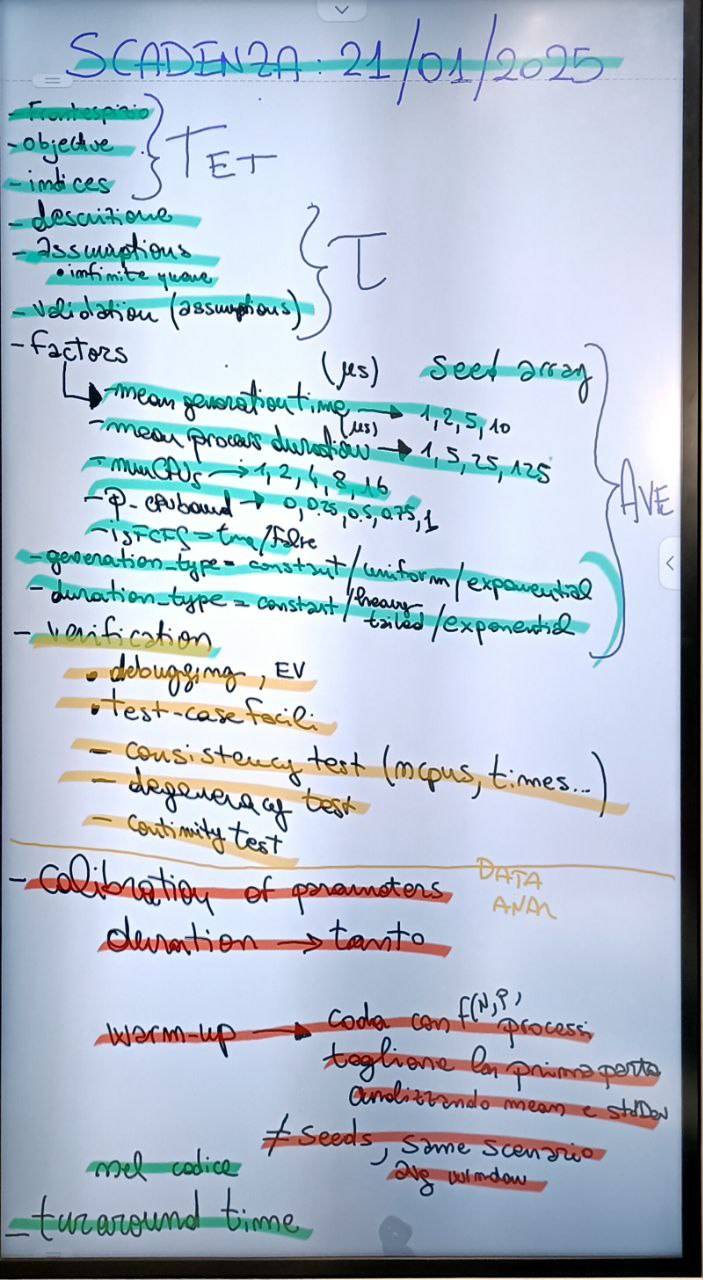
\includegraphics[width=0.6\textwidth]{images/example/pag1.jpeg}
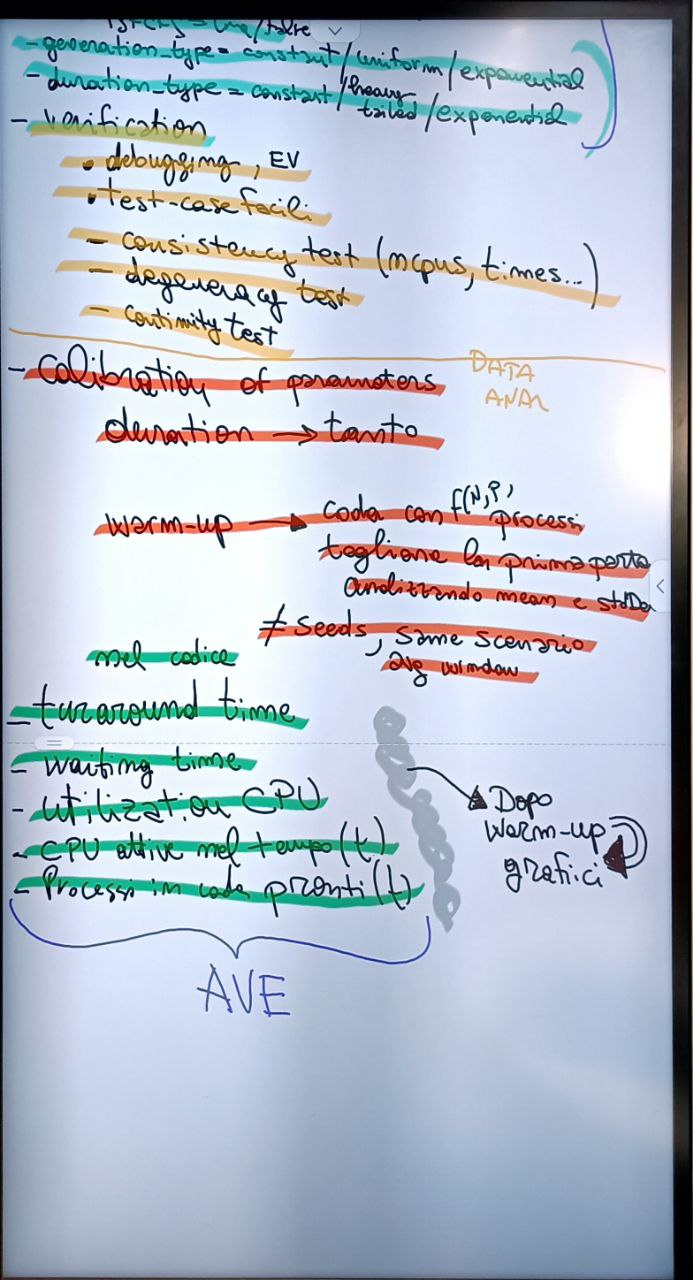
\includegraphics[width=0.6\textwidth]{images/example/pag2.jpeg}
\chapter{Introduction}

\chapter{Design}

\section{Actors}

The application is designed to support three main categories of actors: \textit{Guests}, \textit{Registered Users}, and \textit{Administrators}. Each actor plays a specific role within the system and interacts with the academic content and functionalities according to a well-defined set of permissions and responsibilities.

\subsection{Guest User}
Guests represent users who access the platform without creating an account. They interact with the system in a read-only mode, making use of its core functionalities to explore academic content. A guest can search for academic papers and authors by keywords, view detailed publication records, and access publicly available metadata such as abstracts, citation counts, co-authorship networks, and institutional affiliations. They can also explore statistics aggregated over time, view rankings of authors or institutions by number of publications or citations, and compute author collaboration distances. Although guests can navigate a large part of the platform and gain meaningful insights from the data, they lack any capability for personalization, content contribution, or user-specific recommendations.

\subsection{Registered User}
Registered users are individuals who have created a personal account on the platform. In addition to all the capabilities granted to guests, they benefit from a personalized experience that includes following authors, receiving updates about new publications, and accessing recommendation systems tailored to their interests. A distinctive feature of registered users is the possibility to associate their account with an existing author profile. Once such a link is established the user can actively manage their academic profile. This includes updating their biography, modifying institutional affiliations, and uploading newly published papers. Thus, the registered user may operate either as a general reader of the platform or as an academic contributor, participating in the enrichment of the underlying database.

\subsection{Administrator}
Administrators are a specialized type of User who are entrusted with the management and oversight of the entire platform. Their responsibilities extend beyond personal usage, as they maintain the consistency, reliability, and growth of the system. Administrators can perform operations that affect the global state of the database, including the creation, modification, and deletion of papers, authors, institutions, and publication venues. They also supervise user accounts, manage role assignments, and validate the links between user accounts and author profiles. Furthermore, they have privileged access to global analytics and internal statistics, which support both quality assurance and strategic development of the platform. Administrators ensure the platform remains a reliable and authoritative tool for academic discovery.


\chapter{Conclusions}


% Cite sources that are not cited in the text
% \nocite{*}
\printbibliography

\end{document}

%----------------------------------------------------
